\chpt{Conclusion and future work}\label{chpt:discussion}

This dissertation presents three projects related to human microbiome. The first project presents the Penn microbiome study of pediatric Crohn’s disease. By analyzing the microbiome data and clinical data from a prospective cohort of pediatric Crohn’s disease patients, we revealed the full complement and dynamics of bacteria and fungi associated with Crohn’s disease and treatment. The second project proposes a multi-sample Poisson model to quantify microbial abundances based on the shotgun metagenomic data. The third project presents another statistical model for association analysis of longitudinal microbiome data. The work provides new insight into the role of human gut microbiome in Crohn’s disease. The statistical models proposed in this dissertation also provide new computational tools for microbiome data analysis. However, microbiome is still a relative new and challenging research area. Following are some future work that need further explore.

\section{Integration of metabolomic data with metagenomic data to further understand Crohn's disease}
The work presented in the dissertation focuse on analysis of microbiome data in order to understand the dysbiosis in Crohn's disease. We have demonstrated that the dysbiosis is caused by multiple factors such as inflammation, antibiotic use and diet. However, the detailed mechanism of dysbiosis development in Crohn's disease is still undetermined. In order to address this question, we also generated metabolomic data from the fecal same samples in the previous study. 
Figure~\ref{F54_Metabolites_Heatmap} shows a global profile of the metabolites in control and Crohn's disease samples.  The clustering of samples and metabolites shows some interesting patterns. For example, the carnitines such as C5 carnitine and C9 carnitine are positively correlated with disease status (control vs. Crohn) and disease activity indicated by FCP values.  We applied the Random Forest model to predict the control and Crohn's disease samples with known metabolite abundance (Figure~\ref{F53_Metabolites_RF}). The out-of-bag prediction accuracy is 89\% and the most important metabolites are lipids as well as carnitines. These preliminary results from the metabolomic data analysis indicate that the lipids especially carnitines may play critical role in dysbiosis in Crohn's disease. By integrating metabolomic data with metagenomic data such as microbial abundance and gene pathway abundance, as well as clinical data, we can investigate the association among metabolites, bacteria, fungus, disease activity. It is interesting to know how this association can shed light on novel diagnostic and therapeutic procedures for Crohn's disease. 


\begin{figure*}[hp]
\centering
{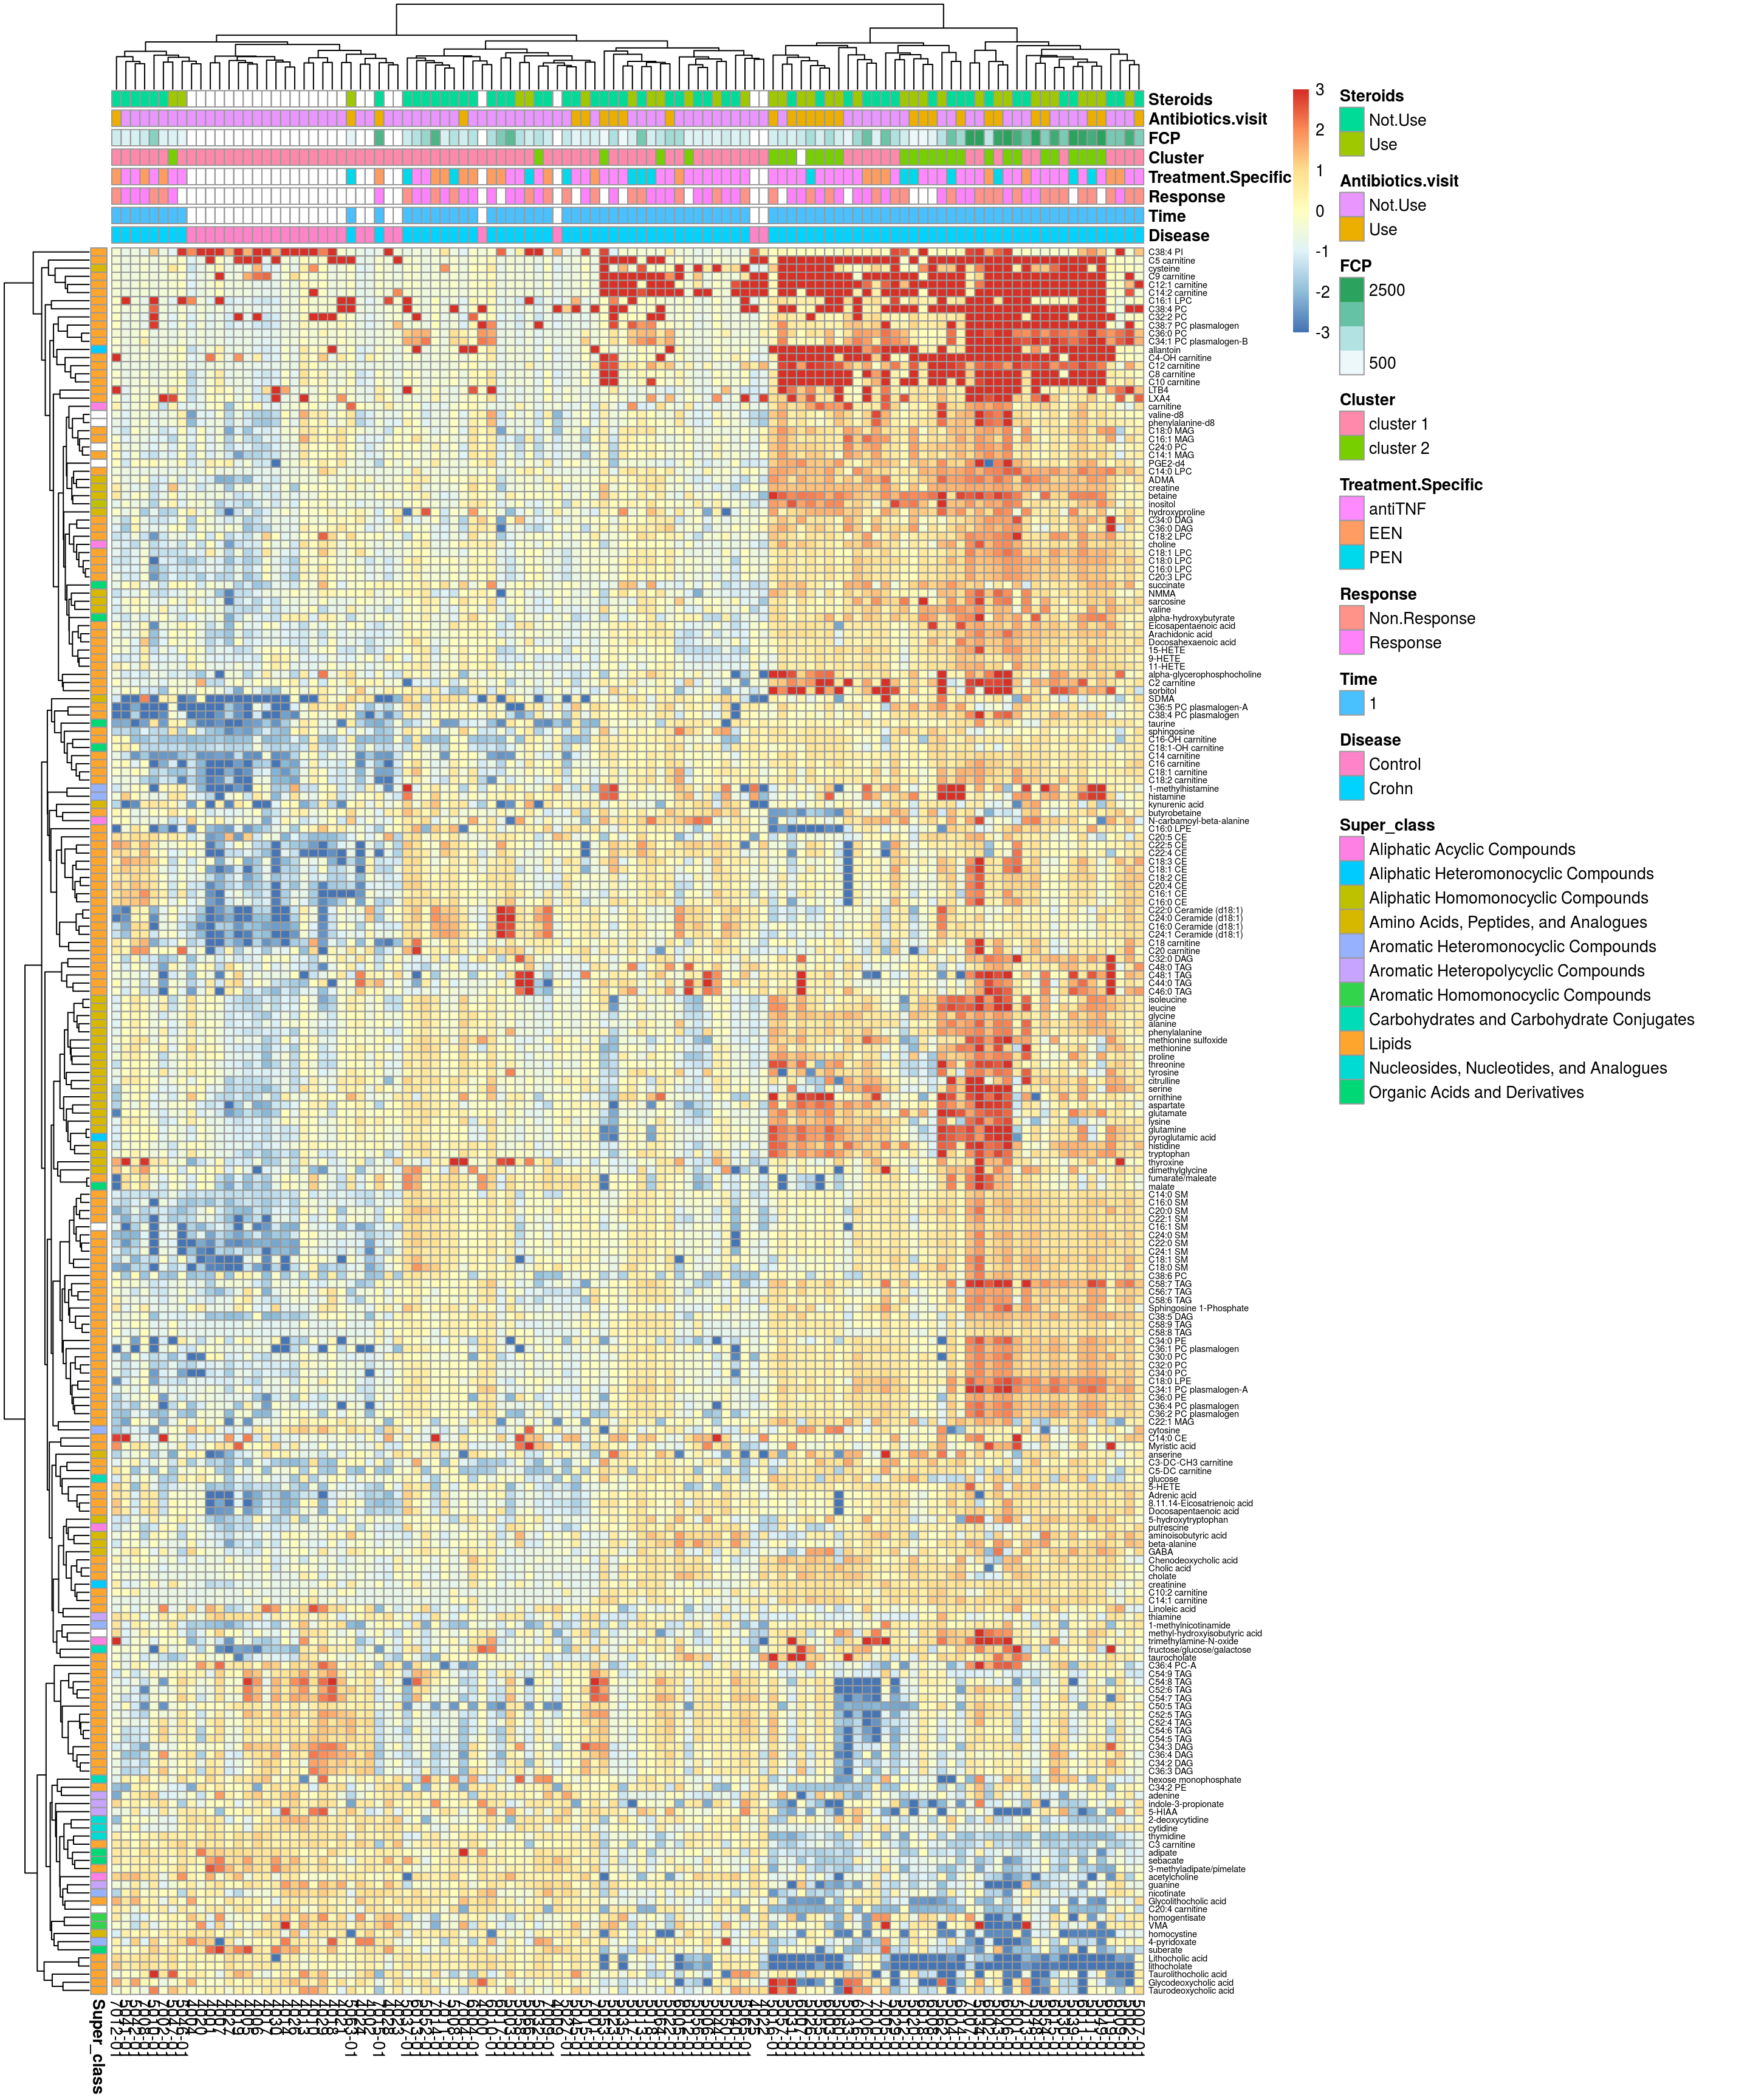
\includegraphics[scale=0.4,trim=0 0 0 0,clip]{Figure/F54_Metabolites_Heatmap.png}
}
\caption[A heatmap demonstrating the relative abundance of known metabolites]{A heatmap demonstrating the relative abundance of known metabolites in control and disease samples at baseline. Metadata are indicated by the color code at the top of the figure. The metabolites are grouped into several classes and indicated by the color code on the left side of the figure. Only metabolites that show differential abundance between control and disease samples at baseline are plotted in the heatmap, which are defined by q value $<$ 0.05 with Wilcoxon rank-sum test}
\label{F54_Metabolites_Heatmap}
\end{figure*}



\begin{figure*}[hp]
\centering
{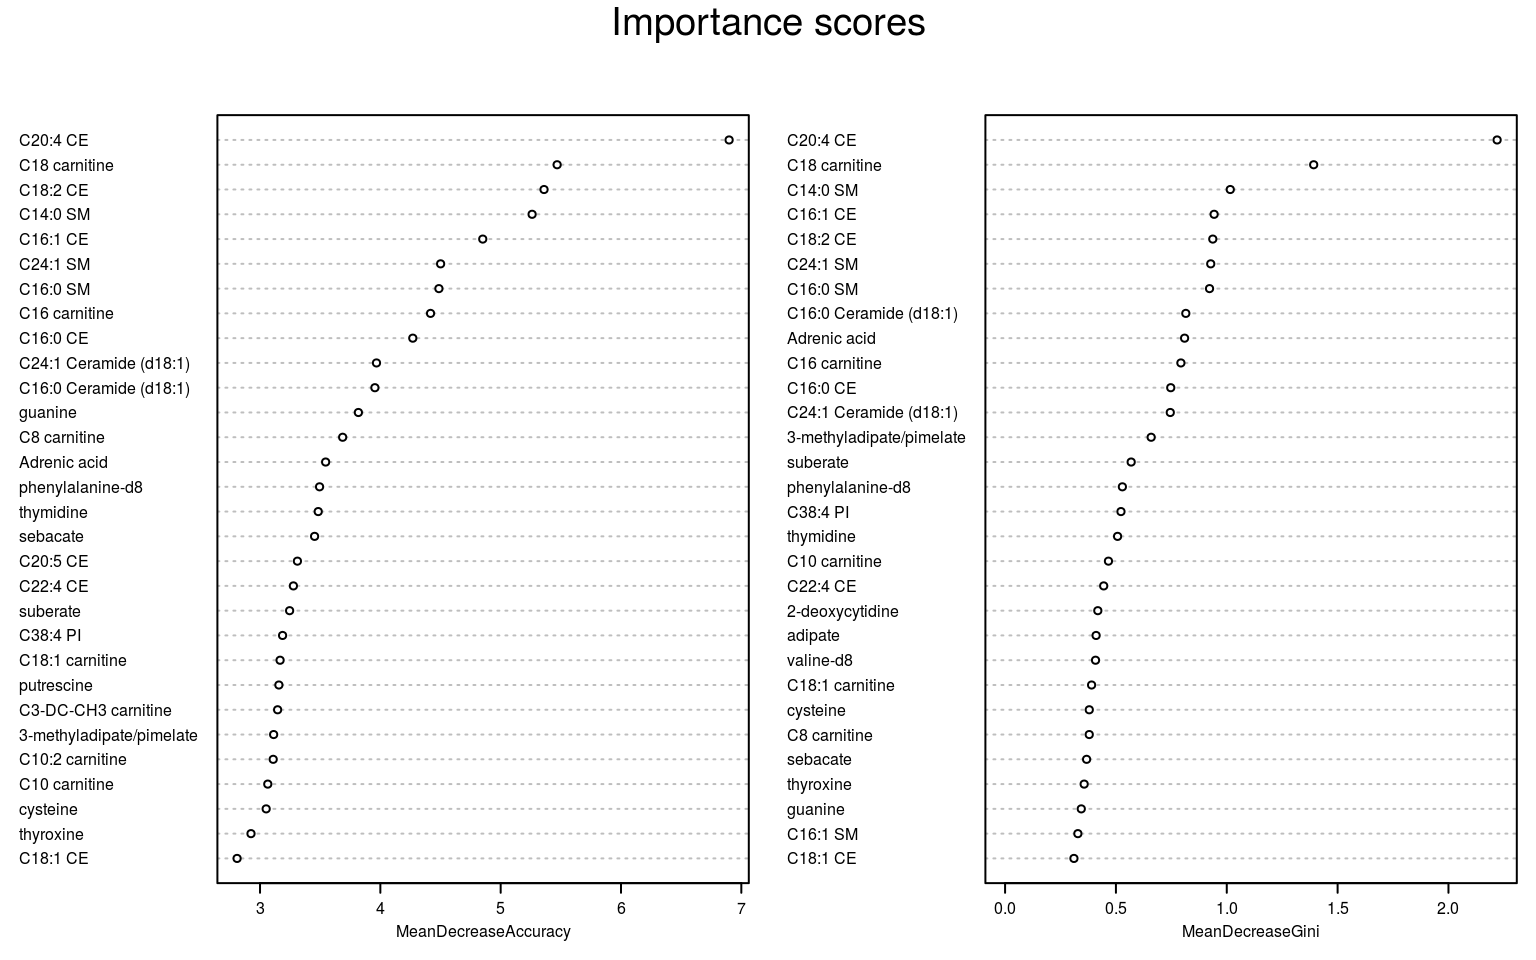
\includegraphics[scale=1.2,trim=0 0 290 30,clip]{Figure/F53_Metabolites_RF.png}
}
\caption[Prediction of control and Crohn's disease samples using known metabolites by Random Forest]{Prediction of control and Crohn's disease samples using known metabolites by Random Forest. The metabolites are ranked by Random Forest so that the top ones are most important in predicting control versus disease samples. Control and Crohn's disease samples at baseline were used in the Random Forest analysis. 
}
\label{F53_Metabolites_RF}
\end{figure*}


\section{Analysis of microbiome data with k-mers} 
The shotgun metagenomic data is challenging to analyze because many similar microbial genomes are presented in the sample and thus it is difficult to sort the sequencing reads back to the reference genome. Currently, the most popular approach for shotgun metagenomic data analysis is to utilize marker genes, either taxa specific markers or universal markers, as alignment reference. This approach has been well adapted and widely applied in shotgun metagenomic studies. However, since those markers are only a small subset of the microbial genomes, thus only a small proportion of the sequencing reads can be aligned to the markers. Thus majority of the data are discarded because they are originally generated from the non-marker genomic regions. 

One alternative approach for shotgun metagenomic data analysis is to make use of k-mers. That is, we can split the sequencing reads into k-mers, say 6mers, and count the k-mer frequency in the sample. The k-mer frequency could be potentially informative. To test this idea, we generated 6mers from the shotgun metagenomic data used in the previous analysis after removing human reads and low quality reads.  The  frequency of each 6mer was counted and then normalized into relative abundance so that the abundance of all 6mers in one sample sums to one. We then applied Random Forest to predict control and Crohn's disease samples using 6mer relative abundance. The out of bag prediction accuracy is 85\% using 6mers and the top six 6mers that are most important to prediction accuracy are plotted in Figure~\ref{F55_Kmer_Difference}. The 6mers such as TACAAC and AAGCTT show significant differential abundance between control and Crohn's disease samples. It is interesting to further explore why those 6mers are associated with disease status. Testing the association between the 6mer abundance and other clinical variables such as FCP values and response status to the treatments is another future research direction. 

More advanced and rigorous statistical models need to be developed for the analysis of k-mers from shotgun metagenomic data. One possible research direction is to apply the topic model on k-mer data. The topic model is a class of statistical models to identify the hidden topics in a collection of documents. In this case, we can consider each sample as a document and k-mers as words in the document. By using topic models, we can identify the hidden biological structure in the data. 

\citet{taddy2013multinomial} introduced a multinomial inverse regression to model the word frequency in the document and derive low dimension representations.
\begin{equation*}
X_y \sim Multinomial(q_y,m_y),
\end{equation*}
where $q_{yj} = \frac{exp(\alpha_j+\beta_jy)}{\sum_{l=1}^{p}exp(\alpha_l+\beta_ly)}$,
$m_y = \sum_{i:y_i=y}m_i$.
Here, $y$ is the index for documents and $X_y$ is the word frequency.
The number of unique words in the documents usually is very large and thus we are facing a high dimensional regression problem. The dimensions  can be reduced through sufficient reduction (SR) and it can be calculated as 
\begin{equation*}
z_i = \beta'f_i,
\end{equation*}
where $f_i = \frac{x_i}{m_i}$.
The SR score is shown to correlate with main theme of the data such as restaurant rating score \citep{taddy2013multinomial}. 

We applied the multinomial inverse regression model to the k-mer data generated from control and Crohn's disease samples. We first extracted 6mers from the shotgun sequencing reads after removing human reads and low quality reads and then counted the frequency of each unique 6mer. We fitted the multinomial inverse regression model and calculated the SR score for each samples. Figure~\ref{F51_SR_control_disease} shows that the SR scores generated from 6mer data are associated with disease status. We further stratified  the Crohn's disease samples into antibiotic use and non-use groups (Figure~\ref{F52_SR_control_disease_antibiotics}). The Crohn's disease samples with antibiotic use show higher SR score than control samples and Crohn's disease samples without antibiotic use.

Although it is inspiring  and promising to see the association between SR score summarized from 6mers and clinical variables such as disease status and antibiotic use, there are still many unsolved  issues. First, different from words in the documents, the k-mer data generated from metagenomic data have several unique features.  Due to the sequencing error, the observed k-mers that originate from the same genomic region may have different sequences. Also, the metagenomic data are mixture of sequencing reads from microbial genomes and human genomes. However, none of the currently available topic models take into account those unique features in the metagenomic data. Thus, developing a topic model that handles these problems is quite necessary. Second, the longer the k-mer, the more informative it would be. For example, in the current analysis, we use 6mers. However, longer k-mers such as k=30 are more biologically informative. But k=30 will generate $1.152922\times 10^{18} $ unique 30mer sequences. It is very computationally challenging to model such data. Therefore, statistical models and computational algorithms for analyzing such ultra-high dimensional data are worth exploring. Third, the topic models can identify  topics with corresponding  theme words. In the k-mer case, how to interpret the biological topics and how to functionally  annotate k-mers in each topic are not clear. 

 

\begin{figure*}[p]
	\centering
	{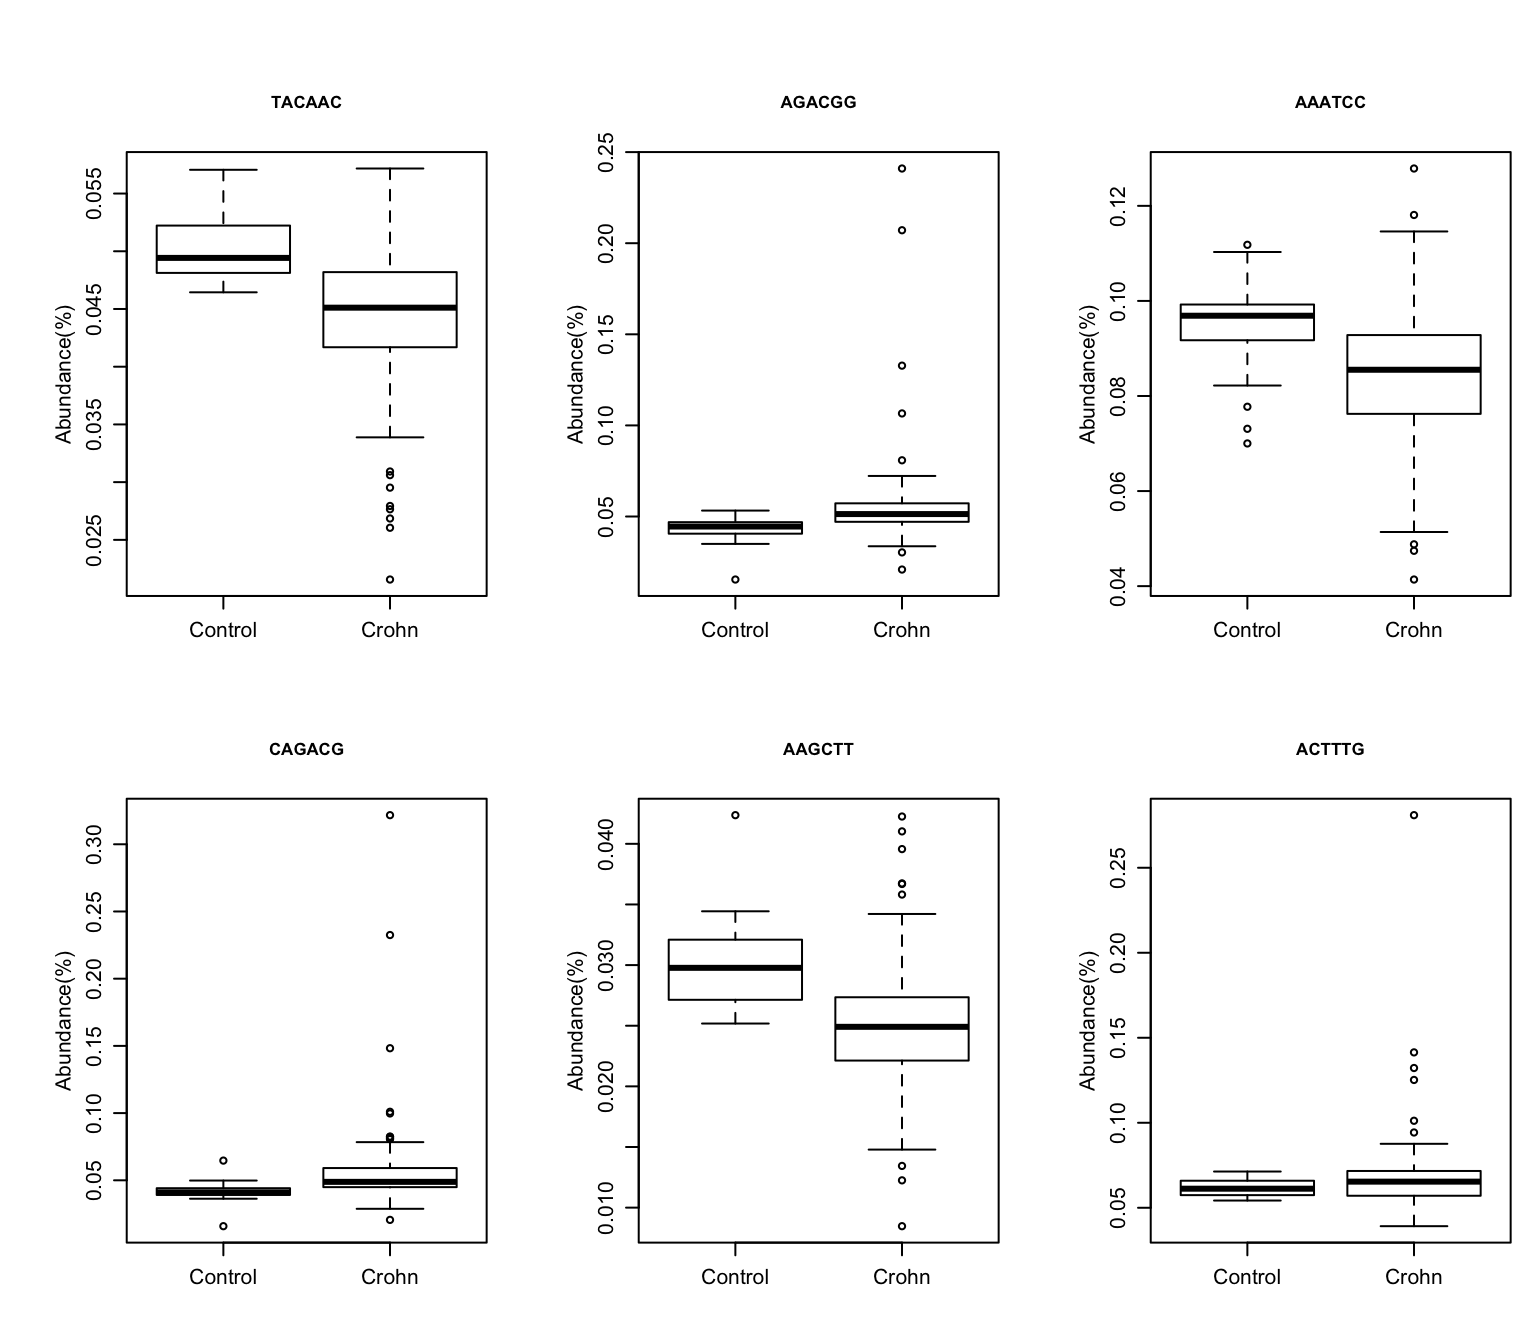
\includegraphics[scale=0.28,trim=40 0 0 0,clip]{Figure/F55_Kmer_Difference.png}
	}
	\caption[Comparison of control and Crohn's disease samples with 6mers]{Comparison of control and Crohn's disease samples with 6mers. The 6mers were generated from the shotgun metagenomic data used in the previous analysis after removing human reads and low quality reads. The  frequencey of each 6mer was counted and then normalized into relative abundance so that the abundance of all 6mers in one sample sums to one. Random Forest was then applied to predict control and Crohn's disease samples using 6mer relative abundance. The top six 6mers that are most important to prediction accuracy are plotted. The 6mer sequences are indicated at the top of each plot.
	}
	\label{F55_Kmer_Difference}
\end{figure*}





\begin{figure*}[p]
\centering
{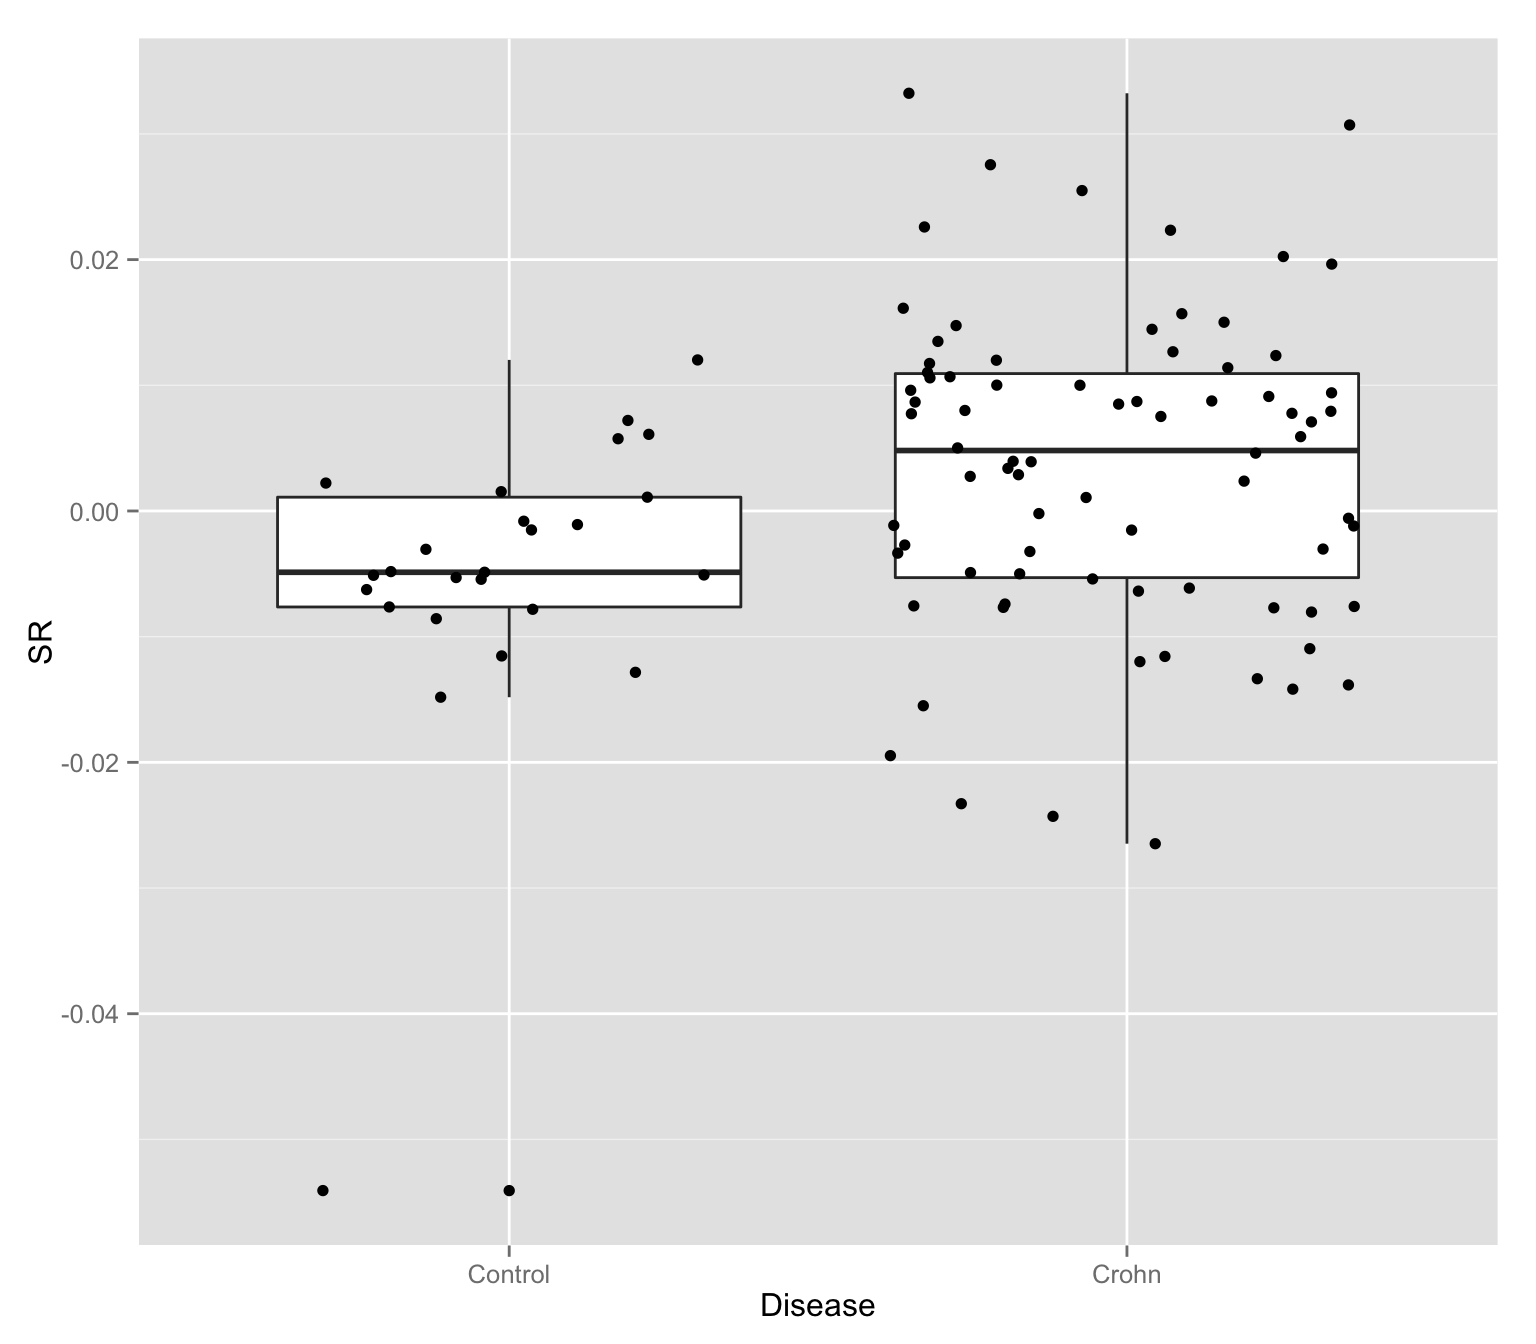
\includegraphics[scale=0.25,trim=0 0 0 0,clip]{Figure/F51_SR_control_disease.png}
}
\caption[Comparison of control and Crohn's disease samples with SR score]{Comparison of control and Crohn's disease samples with SR score. K-mers (k=6) were extracted from the shotgun sequencing reads and the frequency of each k-mer was counted. Then multinomial inverse regression model was fitted to the k-mer count data and the sufficient reduction (SR) score was calculated.   
}
\label{F51_SR_control_disease}
\end{figure*}



\begin{figure*}[p]
\centering
{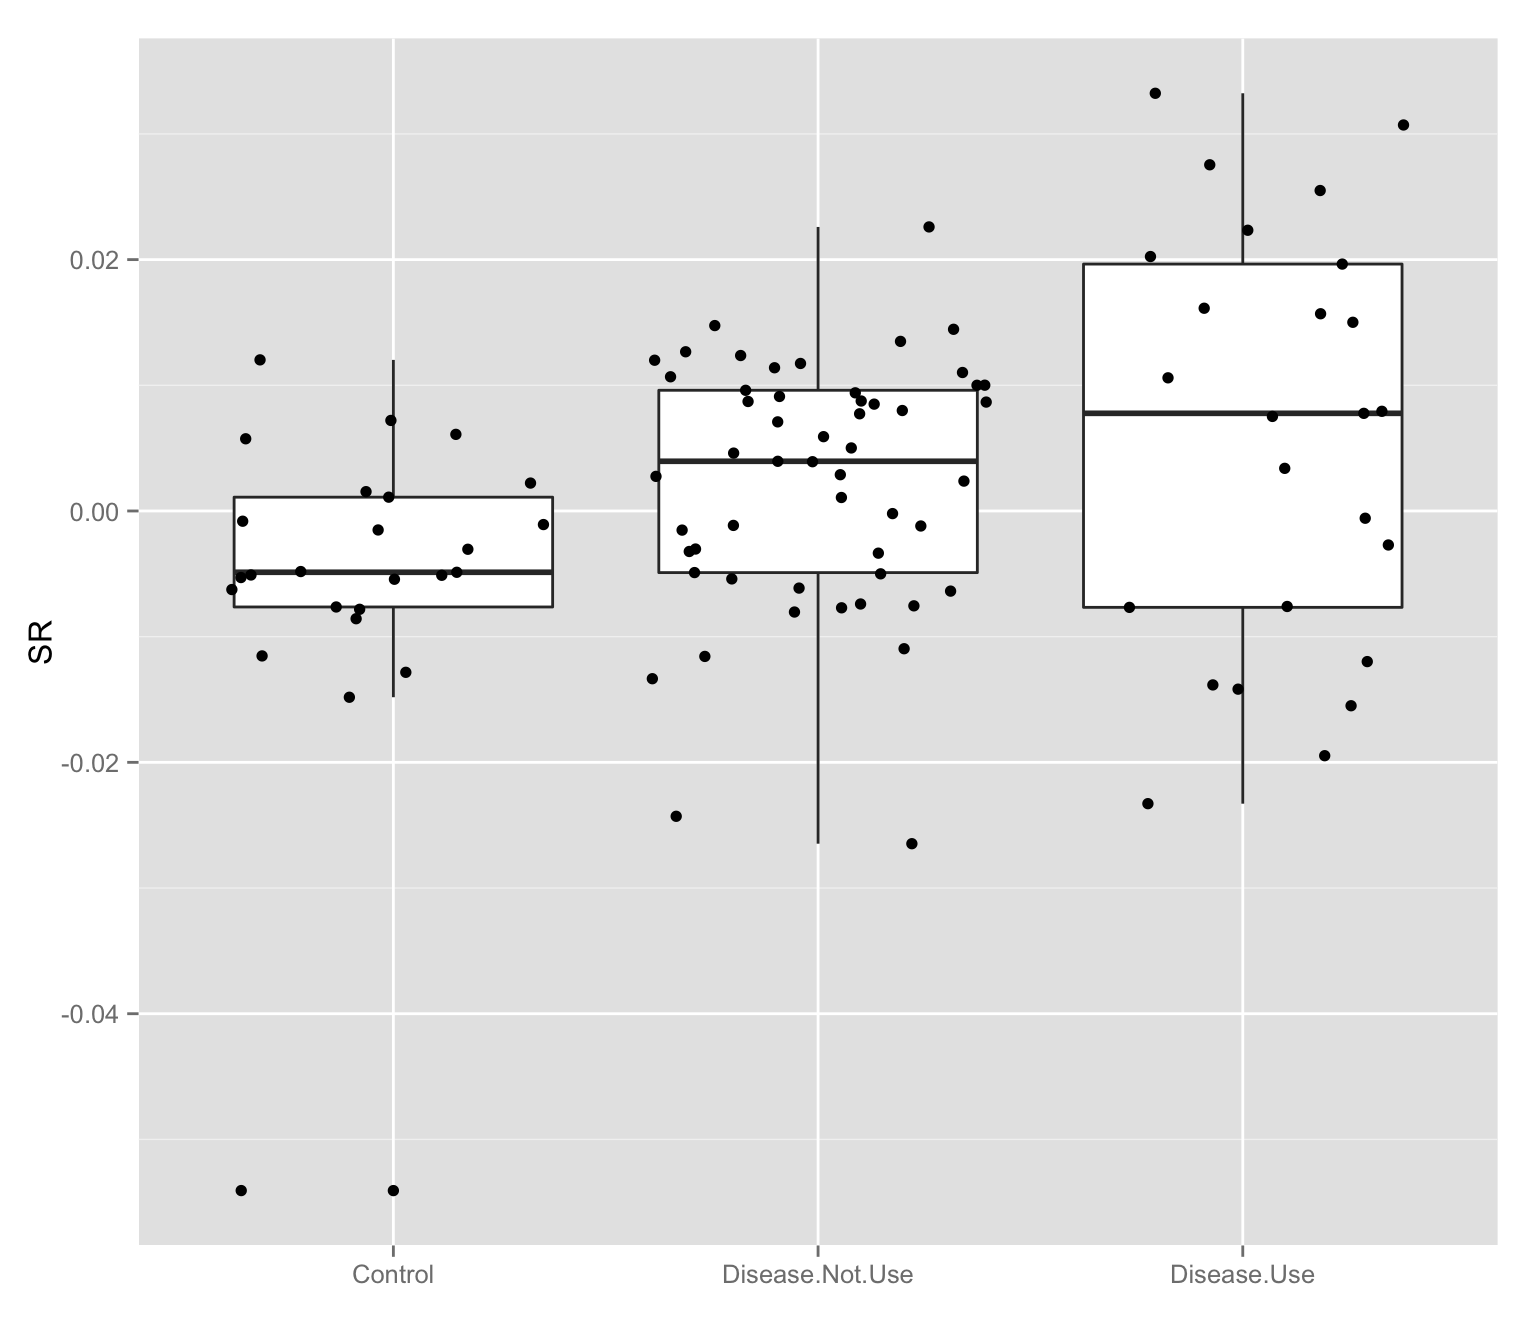
\includegraphics[scale=0.25,trim=0 0 0 0,clip]{Figure/F52_SR_control_disease_antibiotics.png}
}
\caption[Comparison of control and Crohn's disease samples stratified by antibiotic use with SR score]{Comparison of control and Crohn's disease samples stratified by antibiotic use with SR score.  K-mers (k=6) were extracted from the shotgun sequencing reads and the frequency of each k-mer was counted. Then multinomial inverse regression model was fitted to the k-mer count data and the sufficient reduction (SR) score was calculated. 
}
\label{F52_SR_control_disease_antibiotics}
\end{figure*}

In summary, microbiome is still a relative new and challenging research area. More advanced statistical models and efficient computational tools are still needed for metagenomic data analysis. I hope that this dissertation will provide new insight to other researchers in the field. 